% \begin{tikzpicture}[scale=0.85]
\node at (-3.5,2.75) {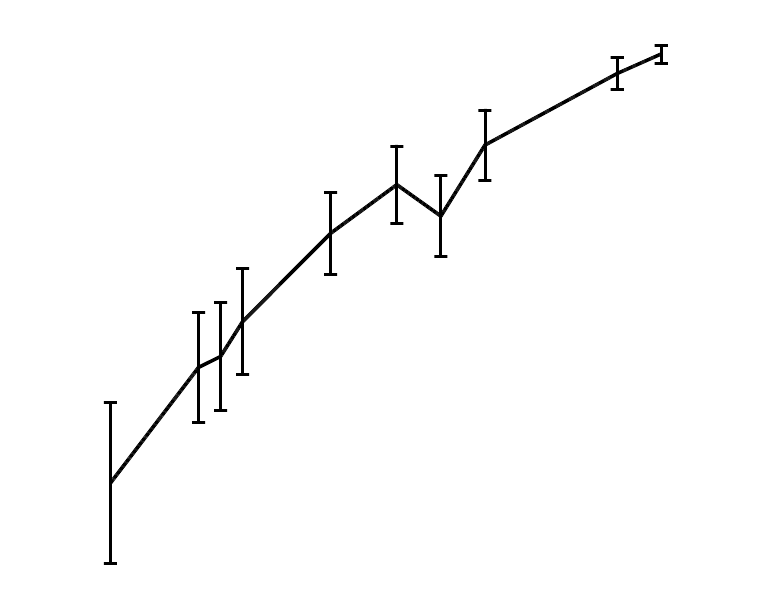
\includegraphics[width=6cm]{img/chap1/reibman2}};
\draw (-7,0) rectangle (0,5.51);
\draw (-7,0.1) -- (-7,0) node[anchor=north] {1};
\draw (-6,0.1) -- (-6,0) node[anchor=north] {1,5};
\draw (-5,0.1) -- (-5,0) node[anchor=north] {2};
\draw (-4,0.1) -- (-4,0) node[anchor=north] {2,5};
\draw (-3,0.1) -- (-3,0) node[anchor=north] {3};
\draw (-2,0.1) -- (-2,0) node[anchor=north] {3,5};
\draw (-1,0.1) -- (-1,0) node[anchor=north] {4};
\draw (0,0.1) -- (0,0) node[anchor=north] {4,5};
\draw (-6.9,0) -- (-7,0) node[anchor=east] {-12};
\draw (-6.9,0.56) -- (-7,0.56) node[anchor=east] {-10};
\draw (-6.9,1.1) -- (-7,1.1) node[anchor=east] {-8};
\draw (-6.9,1.65) -- (-7,1.65) node[anchor=east] {-6};
\draw (-6.9,2.2) -- (-7,2.2) node[anchor=east] {-4};
\draw (-6.9,2.76) -- (-7,2.76) node[anchor=east] {-2};
\draw (-6.9,3.31) -- (-7,3.31) node[anchor=east] {0};
\draw (-6.9,3.87) -- (-7,3.87) node[anchor=east] {2};
\draw (-6.9,4.42) -- (-7,4.42) node[anchor=east] {4};
\draw (-6.9,4.97) -- (-7,4.97) node[anchor=east] {6};
\draw (-6.9,5.51) -- (-7,5.51) node[anchor=east] {8};
\node[below=0.3cm] at (-3.5,0) {Facteur de l'algorithme};
\node[rotate=90] at (-8,2.5) {Qualité subjective relative};
% \end{tikzpicture}